\section{Аналитический раздел}

В данном разделе проводится анализ предметной области, формализуются объекты сцены и рассматриваются математическая модель расчета кинематики шестереночных механизмов. Также производится обзор и сравнительный анализ алгоритмов компьютерной графики для выбора наиболее подходящих алгоритмов в рамках поставленной задачи.

\subsection{Описание и формализация объектов сцены}

Сцена представляет собой трехмерное пространство, содержащее следующие типы объектов.
\begin{enumerate}
	\item Шестерни (зубчатые колеса). Являются основными динамическими объектами. Модель состоит из цилиндрического основания и зубьев, расположенных по окружности. Важными параметрами для построения являются:
	      \begin{itemize}
		      \item $R$ --- радиус делительной окружности;
		      \item $N$ --- количество зубьев (пропорционально радиусу для обеспечения зацепления);
		      \item $h$ --- толщина шестерни;
		      \item $\phi$ --- текущий угол поворота вокруг собственной оси.
	      \end{itemize}
	\item Основание (пол) --- плоскость, на которую проецируются тени объектов. На основании нанесена гексагональная сетка для удобства позиционирования.
	\item Источник света --- бесконечно удаленный объект, задается углом падения и направлением (азимутом) света.
\end{enumerate}

\subsection[Осевая система координат гексагональной сетки]{Осевая система координат гексагональной \\ сетки}
Для позиционирования объектов используется гексагональная сетка. В отличие от прямоугольной сетки, где каждый узел имеет 4 соседа, в гексагональной сетке каждый узел имеет 6 равноудаленных соседей. Эта сетка лучше подходит для размещения шестеренок, так как в данной сетке отсутствуют диагонали.
В отличие от прямоугольной сетки, где оси ортогональны, в гексагональной структуре естественным образом выделяются три оси симметрии. Для математического описания такой структуры наиболее удобна кубическая система координат $(x, y, z)$, подчиняющаяся условию $x + y + z = 0$. Однако, поскольку это условие делает одну из координат избыточной, для хранения данных и оптимизации вычислений применяется осевая система координат~\cite{redblob_hex}.

В осевой системе положение любой ячейки (шестерни) задается парой целочисленных координат $(q, r)$:
\begin{itemize}
	\item $q$ --- координата, соответствующая столбцу (направлена под углом $30^\circ$ к горизонтали);
	\item $r$ --- координата, соответствующая ряду (направлена вертикально или под углом, в зависимости от ориентации).
\end{itemize}

Третья (кубическая) координата $s$ при необходимости может быть вычислена неявно по формуле~\eqref{eq:cubic_coord}:
\begin{equation}
	s = -q - r.
	\label{eq:cubic_coord}
\end{equation}

Данная система координат позволяет выполнять операции смещения и поиска соседей с помощью простого сложения векторов, избегая сложных проверок четности строк, свойственных системам со смещением.

Для визуализации сцены необходимо преобразовать дискретные координаты сетки $(q, r)$ в непрерывные мировые координаты $(x_{world}, z_{world})$. В данной работе используется ориентация шестиугольников вершиной вверх. Преобразование осуществляется по формулам~\eqref{eq:hex_to_cartesian}.

\begin{equation}
	\label{eq:hex_to_cartesian}
	\begin{cases}
		x_{world} = S \cdot \sqrt{3} \cdot \left( q + \frac{r}{2} \right), \\
		z_{world} = S \cdot \frac{3}{2} \cdot r,
	\end{cases}
\end{equation}
где $S$ --- размер шестиугольника (радиус описанной окружности, расстояние от центра до вершины).

Обратное преобразование (нахождение ячейки $(q, r)$ по клику мыши в точку $(x, z)$) выполняется путем инверсии матрицы преобразования \eqref{eq:hex_to_cartesian} и последующего округления до ближайшего узла сетки по формуле~\eqref{eq:cartesian_to_hex}.

\begin{equation}
	\begin{cases}
		q_{float} = \frac{\frac{\sqrt{3}}{3} \cdot x_{world} - \frac{1}{3} \cdot z_{world}}{S}, \\
		r_{float} = \frac{\frac{2}{3} \cdot z_{world}}{S}.
	\end{cases}
	\label{eq:cartesian_to_hex}
\end{equation}

После получения вещественных координат $(q_{float}, r_{float})$ применяется алгоритм округления кубических координат для устранения погрешностей дискретизации и выбора корректной ячейки.

\subsection[Математическая модель кинематики механизмов]{Математическая модель кинематики \\ механизмов}

Система сцепленных шестеренок может быть представлена в виде неориентированного графа $G = (V, E)$, где $V$ --- множество шестеренок (вершин), а $E$ --- множество пар сцепленных шестеренок (ребер).

В системе присутствует один источник вращения (ведущая шестерня) с заданной угловой скоростью $\omega_{driver}$. Задача кинематического расчета сводится к определению угловых скоростей $\omega_i$ для всех остальных шестеренок.

Условие отсутствия проскальзывания в точке контакта двух шестеренок $i$ и $j$ требует равенства линейных скоростей их зубьев $v_i$ и $v_j$:
\begin{equation}
	v_i = -v_j.
\end{equation}
Знак минус обусловлен тем, что в паре внешнего зацепления шестерни вращаются в противоположных направлениях.

Связь линейной скорости $v$ и угловой скорости $\omega$ выражается формулой $v = \omega \cdot R$. Следовательно, передаточная функция для двух сцепленных шестеренок с угловыми скоростями $\omega_i$ и $\omega_j$ и радиусами $R_i$ и $R_j$ описывается уравнением~\eqref{eq:transmission_function}~\cite{artobolevsky}.
\begin{equation}
	\omega_j = -\omega_i \cdot \frac{R_i}{R_j}.
	\label{eq:transmission_function}
\end{equation}

Для распространения вращения по всей системе используется алгоритм обхода графа в ширину (BFS).
Алгоритм также должен выполнять проверку на заклинивание. Заклинивание происходит, если в графе существуют циклы, и при обходе обнаруживается, что для одной и той же шестерни приходят противоречивые требования к скорости или направлению вращения от разных соседей. Если для вершины $k$ уже вычислена скорость $\omega_k$, а новый путь от соседа $m$ требует скорости $\omega'_k$, и $|\omega_k - \omega'_k| > \varepsilon$, то система считается заклинившей.

Также для визуальной корректности необходимо учитывать фазовое смещение $\theta$, чтобы зубья одной шестерни попадали во впадины другой. Угол поворота ведомой шестерни радиусом $R_{next}$ и с количеством зубьев $N_{next}$ рассчитывается по формуле~\eqref{eq:offset}.
\begin{equation}
	\theta_{next} = \alpha \cdot (1 + \frac{R_{curr}}{R_{next}}) - \theta_{curr} \cdot \frac{R_{curr}}{R_{next}} + \pi + \frac{\pi}{N_{next}},
	\label{eq:offset}
\end{equation}
где
\begin{itemize}
	\item $\alpha$ --- угол вектора, соединяющего центры шестеренок;
	\item $\theta_{curr}$ --- фазовое смещение текущей шестерни;
	\item $\theta_{next}$ --- фазовое смещение ведомой шестерни;
	\item $R_{curr}$ --- радиус текущей шестерни.
\end{itemize}

\subsection[Математические основы построения трехмерного изображения]{Математические основы построения \\ трехмерного изображения}

Для визуализации трехмерной сцены на двумерном экране используется графический конвейер, включающий последовательность преобразований систем координат~\cite{foley}.

Любая точка $P_{local}$ из локального пространства модели преобразуется в экранные координаты $P_{screen}$ с помощью умножения на матрицы по формуле~\eqref{eq:transform}.
\begin{equation}
	P_{screen} = M_{proj} \cdot M_{view} \cdot M_{model} \cdot P_{local},
	\label{eq:transform}
\end{equation}
где
\begin{enumerate}
	\item Модельная матрица $M_{model}$ отвечает за положение, поворот и масштаб объекта в мировом пространстве. Для вращающейся шестерни эта матрица пересчитывается каждый кадр в зависимости от угла $\phi$.
	\item Видовая матрица $M_{view}$ трансформирует мировые координаты в систему координат камеры. Она определяется позицией наблюдателя, точкой, на которую он смотрит, и вектором <<вверх>>.
	\item Проекционная матрица $M_{proj}$ преобразует усеченную пирамиду видимости в куб нормализованных координат устройства. Для реалистичного отображения используется перспективная проекция, при которой удаленные объекты кажутся меньше. Элементы матрицы зависят от угла обзора и соотношения сторон экрана.
\end{enumerate}

После матричных преобразований производится перспективное деление (деление на координату $w$) и переход к экранным координатам.

\subsection[Анализ алгоритмов удаления невидимых поверхностей]{Анализ алгоритмов удаления невидимых \\ поверхностей}

При отображении трехмерных объектов на двумерном экране необходимо определить, какие части объектов видны наблюдателю, а какие скрыты другими объектами или собственными гранями. Рассмотрим основные методы решения этой задачи.

\subsubsection{Алгоритм Робертса}
Данный алгоритм работает в пространстве объекта и предназначен преимущественно для выпуклых многогранников. Алгоритм состоит из двух этапов.
\begin{enumerate}
	\item Удаление нелицевых граней. Для каждой грани вычисляется скалярное произведение вектора взгляда и внешней нормали к грани. Если результат положительный, грань <<отвернута>> от наблюдателя и отбрасывается.
	\item Сравнение каждого ребра каждого тела с остальными телами. Проверяется, экранируется ли ребро (или его часть) каким-либо другим объектом сцены.
\end{enumerate}
Алгоритм математически точен, но имеет сложность $O(N^2)$, где $N$ --- количество объектов, и плохо масштабируется для сложных сцен с невыпуклыми объектами (требует разбиения на выпуклые части)~\cite{rogers1989}.

\subsubsection{Алгоритм художника}
Алгоритм работает в пространстве объекта и изображения. Суть заключается в сортировке всех полигонов сцены по их глубине (расстоянию от наблюдателя). Отрисовка происходит в порядке от самых дальних полигонов к самым ближним. Ближние объекты перекрывают дальние в буфере кадра.
Главный недостаток алгоритма --- невозможность корректной обработки случаев циклического перекрытия (полигон A перекрывает B, B перекрывает C, C перекрывает A) и случаев взаимопересечения полигонов без их предварительного геометрического разбиения~\cite{rogers1989}.

\subsubsection{Алгоритм обратной трассировки лучей}
Метод работает в пространстве изображения. Для каждого пикселя экрана из центра проекции (глаза наблюдателя) выпускается луч. Находится ближайшая точка пересечения луча с объектами сцены. Цвет пикселя определяется свойствами объекта в точке пересечения.
Алгоритм автоматически решает проблему видимости, теней и отражений. Однако он требует больших вычислительных затрат, так как поиск пересечений должен выполняться для каждого пикселя с каждым полигоном~\cite{shikin2005}.

\subsubsection{Алгоритм, использующий Z-буфер}
Работает в пространстве изображения. Помимо буфера цвета, используется буфер глубины (Z-Buffer) той же размерности. В ячейках Z-буфера хранятся значения глубины (координаты $z$ или $1/z$) ближайшего к наблюдателю объекта, спроецированного в данный пиксель~\cite{rtr4}.
Алгоритм состоит из следующих этапов.
\begin{enumerate}
	\item Изначально Z-буфер заполняется значением бесконечности (максимальной глубины).
	\item При растеризации каждого полигона для каждого пикселя вычисляется его глубина $z_{current}$.
	\item Сравнивается $z_{current}$ со значением $z_{buffer}$, уже хранящимся в буфере.
	\item Если $z_{current} < z_{buffer}$, то пиксель ближе к наблюдателю: цвет записывается в буфер кадра, а $z_{buffer}$ обновляется значением $z_{current}$.
\end{enumerate}

\subsubsection{Сравнение алгоритмов удаления невидимых поверхностей}

Сравнение алгоритмов удаления невидимых поверхностей представлено в таблице~\ref{table:hsr}, где N --- количество объектов, n --- количество пикселей.
\begin{table}[h!]
	\caption{Сравнение алгоритмов удаления невидимых поверхностей}
	\label{table:hsr}
	\begin{tabular}{|p{3.3cm}|p{2.5cm}|p{3.2cm}|p{5cm}|}
		\hline
		Алгоритм          & Сложность      & Использование памяти & Ограничения                                \\ \hline
		Робертса          & $O(N^2)$       & $O(N)$               & Только выпуклые тела, сложность реализации \\ \hline
		Художника         & $O(N \log N)$  & $O(N)$               & Циклические перекрытия, пересечения        \\ \hline
		Трассировка лучей & $O(n \cdot N)$ & $O(N)$               & Очень низкая скорость без оптимизации      \\ \hline
		Z-буфер           & $O(n \cdot N)$ & $O(N + n)$           & Требует доп. памяти, возможен Z-fighting   \\ \hline
	\end{tabular}
\end{table}

Для выполнения работы выбран алгоритм, использующий Z-буфер. Он позволяет корректно отображать пересекающиеся объекты (ось, проходящая сквозь шестерню), прост в реализации при программной растеризации и имеет линейную зависимость времени работы от количества обрабатываемых фрагментов.

\subsection{Анализ моделей освещения и закраски}

Для придания трехмерным объектам объема и реалистичности необходимо рассчитывать взаимодействие света с поверхностью.

\subsubsection{Плоская закраска}
Вектор нормали вычисляется один раз для всего полигона (как векторное произведение двух его сторон). Освещенность рассчитывается для этого вектора, и весь полигон закрашивается одним цветом.
Метод очень быстр, но дает изображение с четко видимыми гранями (<<фасеточная>> структура). Это подходит для стилизованной графики, но плохо передает кривизну поверхностей~\cite{shikin2005}.

\subsubsection{Закраска Гуро}
Нормали задаются в вершинах полигона. Освещенность рассчитывается для каждой из трех вершин. Затем полученные цвета линейно интерполируются по поверхности треугольника в процессе растеризации.
Метод позволяет сгладить грани, но имеет существенный недостаток: зеркальные блики рассчитываются некорректно. Если блик попадает в центр полигона, а вершины освещены слабо, блик просто исчезнет~\cite{porev2002}.

\subsubsection{Закраска Фонга}
Наиболее качественный метод локального освещения. В вершинах задаются нормали. В процессе растеризации между вершинами интерполируются векторы нормалей. Освещение рассчитывается для каждого пикселя на основе интерполированной нормали.
Модель освещения Фонга включает три компоненты и считается по формуле~\eqref{eq:phong}~\cite{rogers1989}.
\begin{equation}
	I = I_{ambient} + I_{diffuse} \cdot (\vec{L} \cdot \vec{N}) + I_{specular} \cdot (\vec{R} \cdot \vec{V})^n,
	\label{eq:phong}
\end{equation}
где
\begin{itemize}
	\item $I_{ambient}$ --- фоновое освещение;
	\item $I_{diffuse}$ --- рассеянное освещение;
	\item $I_{specular}$ --- зеркальное освещение;
	\item $n$ --- показатель гладкости материала;
	\item $\vec{N}$ --- нормаль;
	\item $\vec{L}$ --- вектор на свет;
	\item $\vec{R}$ --- вектор отражения;
	\item $\vec{V}$ --- вектор на наблюдателя.
\end{itemize}
Метод дает качественные блики на криволинейных поверхностях.

\subsubsection{Сравнение методов закраски}

Пример работы методов закраски представлен на рисунке~\ref{fig:shading_example}.

\begin{figure}[h!]
	\centering
	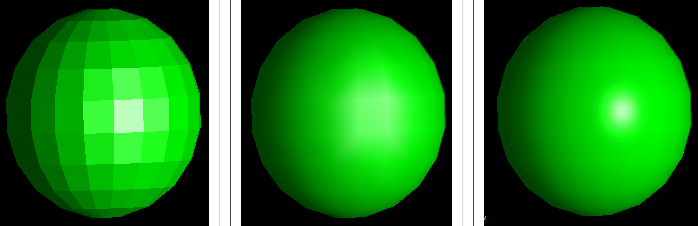
\includegraphics[width=0.8\textwidth]{img/shadingoptions.png}
	\caption{Пример работы методов закраски: слева --- плоская, в центре --- Гуро, справа --- Фонг}
	\label{fig:shading_example}
\end{figure}

Сравнение методов закраски представлено в таблице~\ref{table:shading}.

\begin{table}[h!]
	\caption{Сравнение методов закраски}
	\label{table:shading}
	\begin{tabular}{|p{3cm}|p{4cm}|p{6cm}|}
		\hline
		Метод   & Качество бликов & Вычислительные затраты \\ \hline
		Плоская & Отсутствуют     & Минимальные            \\ \hline
		Гуро    & Низкое          & Средние                \\ \hline
		Фонга   & Высокое         & Высокие                \\ \hline
	\end{tabular}
\end{table}

Для выполнения работы выбрана закраска Фонга, так как она позволяет максимально реалистично отображать блики.

\subsection{Анализ методов построения теней}

Тени являются важнейшим пространственным ориентиром, позволяющим оценить положение объектов.

\subsubsection{Теневые карты}
Алгоритм требует двух проходов рендеринга. Сначала сцена рендерится с точки зрения источника света, сохраняя только глубину. Затем, при основном рендеринге, координаты каждого пикселя преобразуются в пространство света и сравниваются с картой глубины.
Метод универсален (тени падают на любые объекты), но подвержен артефактам дискретизации (<<лесенки>> на краях теней) и сложен в реализации~\cite{porev2002}.

\subsubsection{Теневые объемы}
Геометрический метод, основанный на построении усеченных пирамид, образованных силуэтом объекта и источником света. Использует буфер трафарета для подсчета вхождений пикселя в объем тени. Дает идеально четкие края, но требует больших затрат на геометрические вычисления и сложен для моделей с большим количеством полигонов~\cite{rtr4}.

\subsubsection{Планарная проекция}
Метод применим, когда тени нужно отбрасывать только на плоскую поверхность. Геометрия объекта <<сплющивается>> на плоскость пола с помощью матрицы проекции $M_{shadow}$, которая зависит от положения источника света и уравнения плоскости. Сплющенная геометрия отрисовывается темным цветом без записи в Z-буфер.
Матрица проекции на плоскость $y=0$ для направленного света $\vec{L}$ вычисляется по формуле~\eqref{eq:shadow_matrix}.
\begin{equation}
	M_{shadow} = \begin{pmatrix}
		1 & -L_x/L_y & 0 & 0 \\
		0 & 0        & 0 & 0 \\
		0 & -L_z/L_y & 1 & 0 \\
		0 & 0        & 0 & 1
	\end{pmatrix}.
	\label{eq:shadow_matrix}
\end{equation}

\subsubsection{Сравнение методов построения теней}

Сравнение методов построения теней представлено в таблице~\ref{table:shadows}

\begin{table}[h!]
	\centering
	\caption{Сравнение методов построения теней}
	\label{table:shadows}
	\begin{tabular}{|p{3.4cm}|p{4cm}|p{2.5cm}|p{3.5cm}|}
		\hline
		Метод              & Область применения  & Качество краев & Производитель-ность         \\ \hline
		Теневые карты      & Универсальный       & Низкое         & Зависит от разрешения карты \\ \hline
		Теневые объемы     & Универсальный       & Высокое        & Низкая                      \\ \hline
		Планарная проекция & Только на плоскость & Высокое        & Высокая                     \\ \hline
	\end{tabular}
\end{table}

Для выполнения работы выбран метод планарной проекции. В задаче визуализации настольного механизма тени падают исключительно на плоскость основания (стол). Этот метод обеспечивает высокую производительность и отличное качество краев тени.

\subsection*{Вывод}

На основе проведенного анализа для реализации выбраны следующие методы:
\begin{itemize}
	\item Удаление невидимых поверхностей: Алгоритм Z-буфера, обеспечивающий корректную обработку пересекающейся геометрии.
	\item Освещение: Модель Фонга с попиксельным расчетом для качественной передачи металлических бликов.
	\item Тени: Планарная проекция на плоскость основания, как наиболее эффективный метод для данной постановки задачи.
	\item Кинематика: Графовый подход с поиском в ширину для распространения вращения и детектирования коллизий.
\end{itemize}
